\chapter{Die Anforderungsdefinition}
Dieses Kapitel soll durch Untersuchung helfen, Vorstellung für die Anforderungen an Ampelhinweissystem -App zu bekommen. 
Im heutigen High-Technologie Zeitalter ist gerade die Benutzbarkeit bei der Entwicklung eines Produktes ein wichtiger Faktor, der von Software-Entwicklern beachtet werden muss. Die Anforderungen der Nutzer stehen dabei im Mittelpunkt. Es geht in erster Linie darum, jene zufrieden zu stellen und nicht nur Interesse, sondern auch Begeisterung beim potentiellen Kunden zu wecken. Verschiedene Methoden, diese Anforderungen besser zu identifizieren und erfüllen zu können, haben sich bereits verbreitet und basieren meistens auf einer präzisen Darstellung der NutzerInnen.
\section{Die graphische Oberfläche}

Hohe Kontraste wegen Wetter
einfache UI 
Minimalistisch sodass ein Blick genügt und man nicht abgelenkt wird.
Angezeigt wird: Geschwindigkeit schneller oder langsamer, 
Restrotanzeige.
\begin{figure}[H]
        \centering
        \begin{subfigure}[t]{0.36\textwidth}
                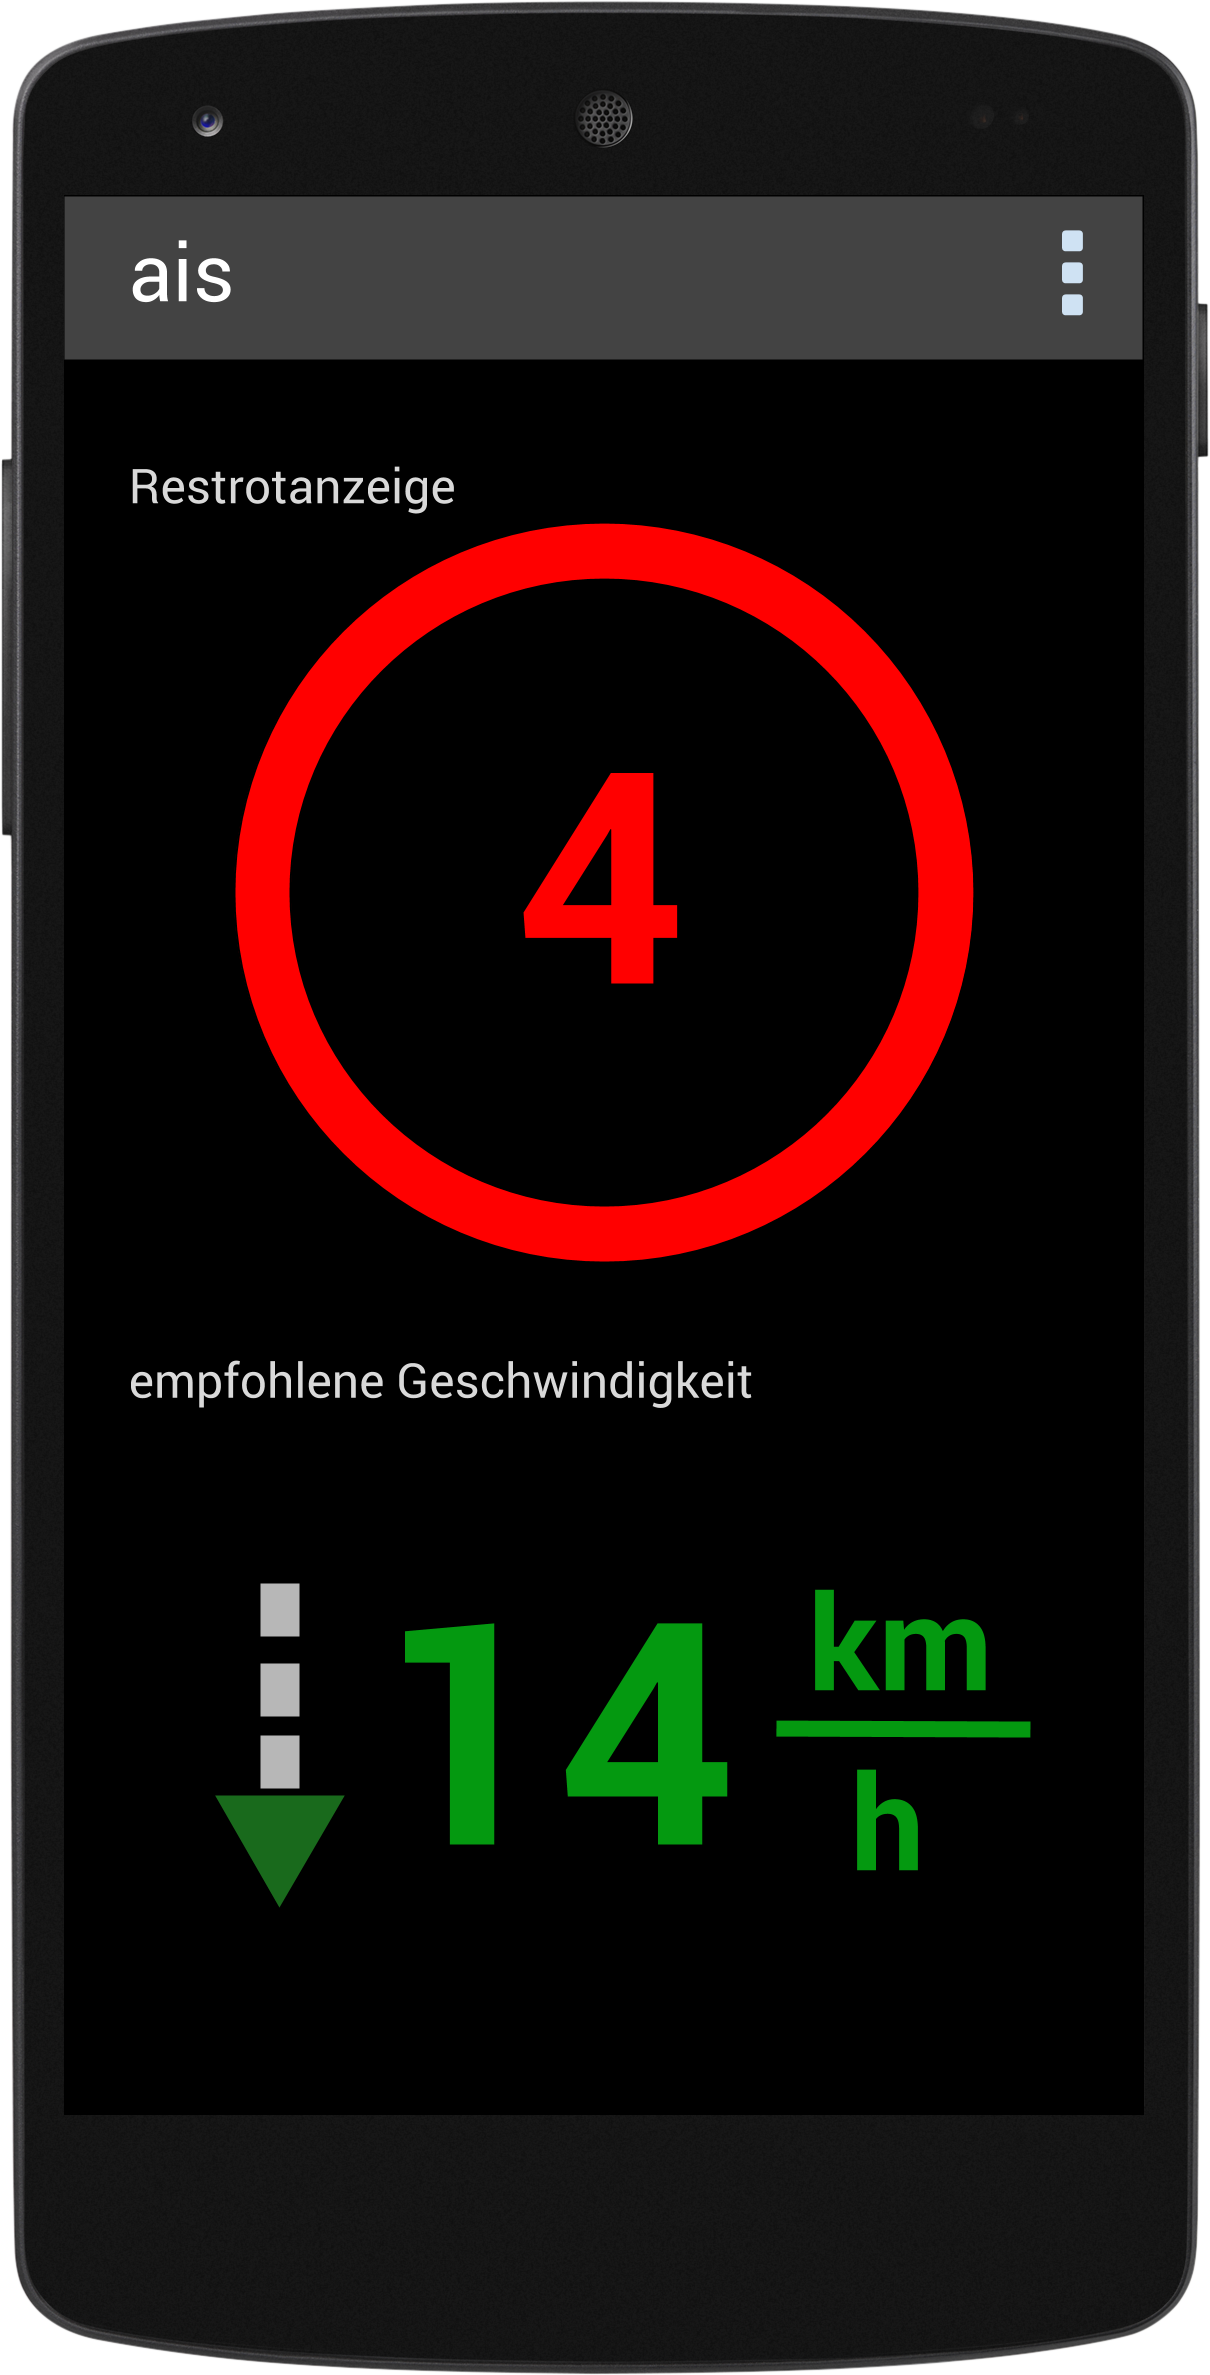
\includegraphics[width=\textwidth]{langsamer}
                \caption[Systemzustand a]{Weiterfahrt durch Verlangsamung möglich}
                \label{fig:langsamer}
        \end{subfigure}
        \hfill
        \begin{subfigure}[t]{0.36\textwidth}
                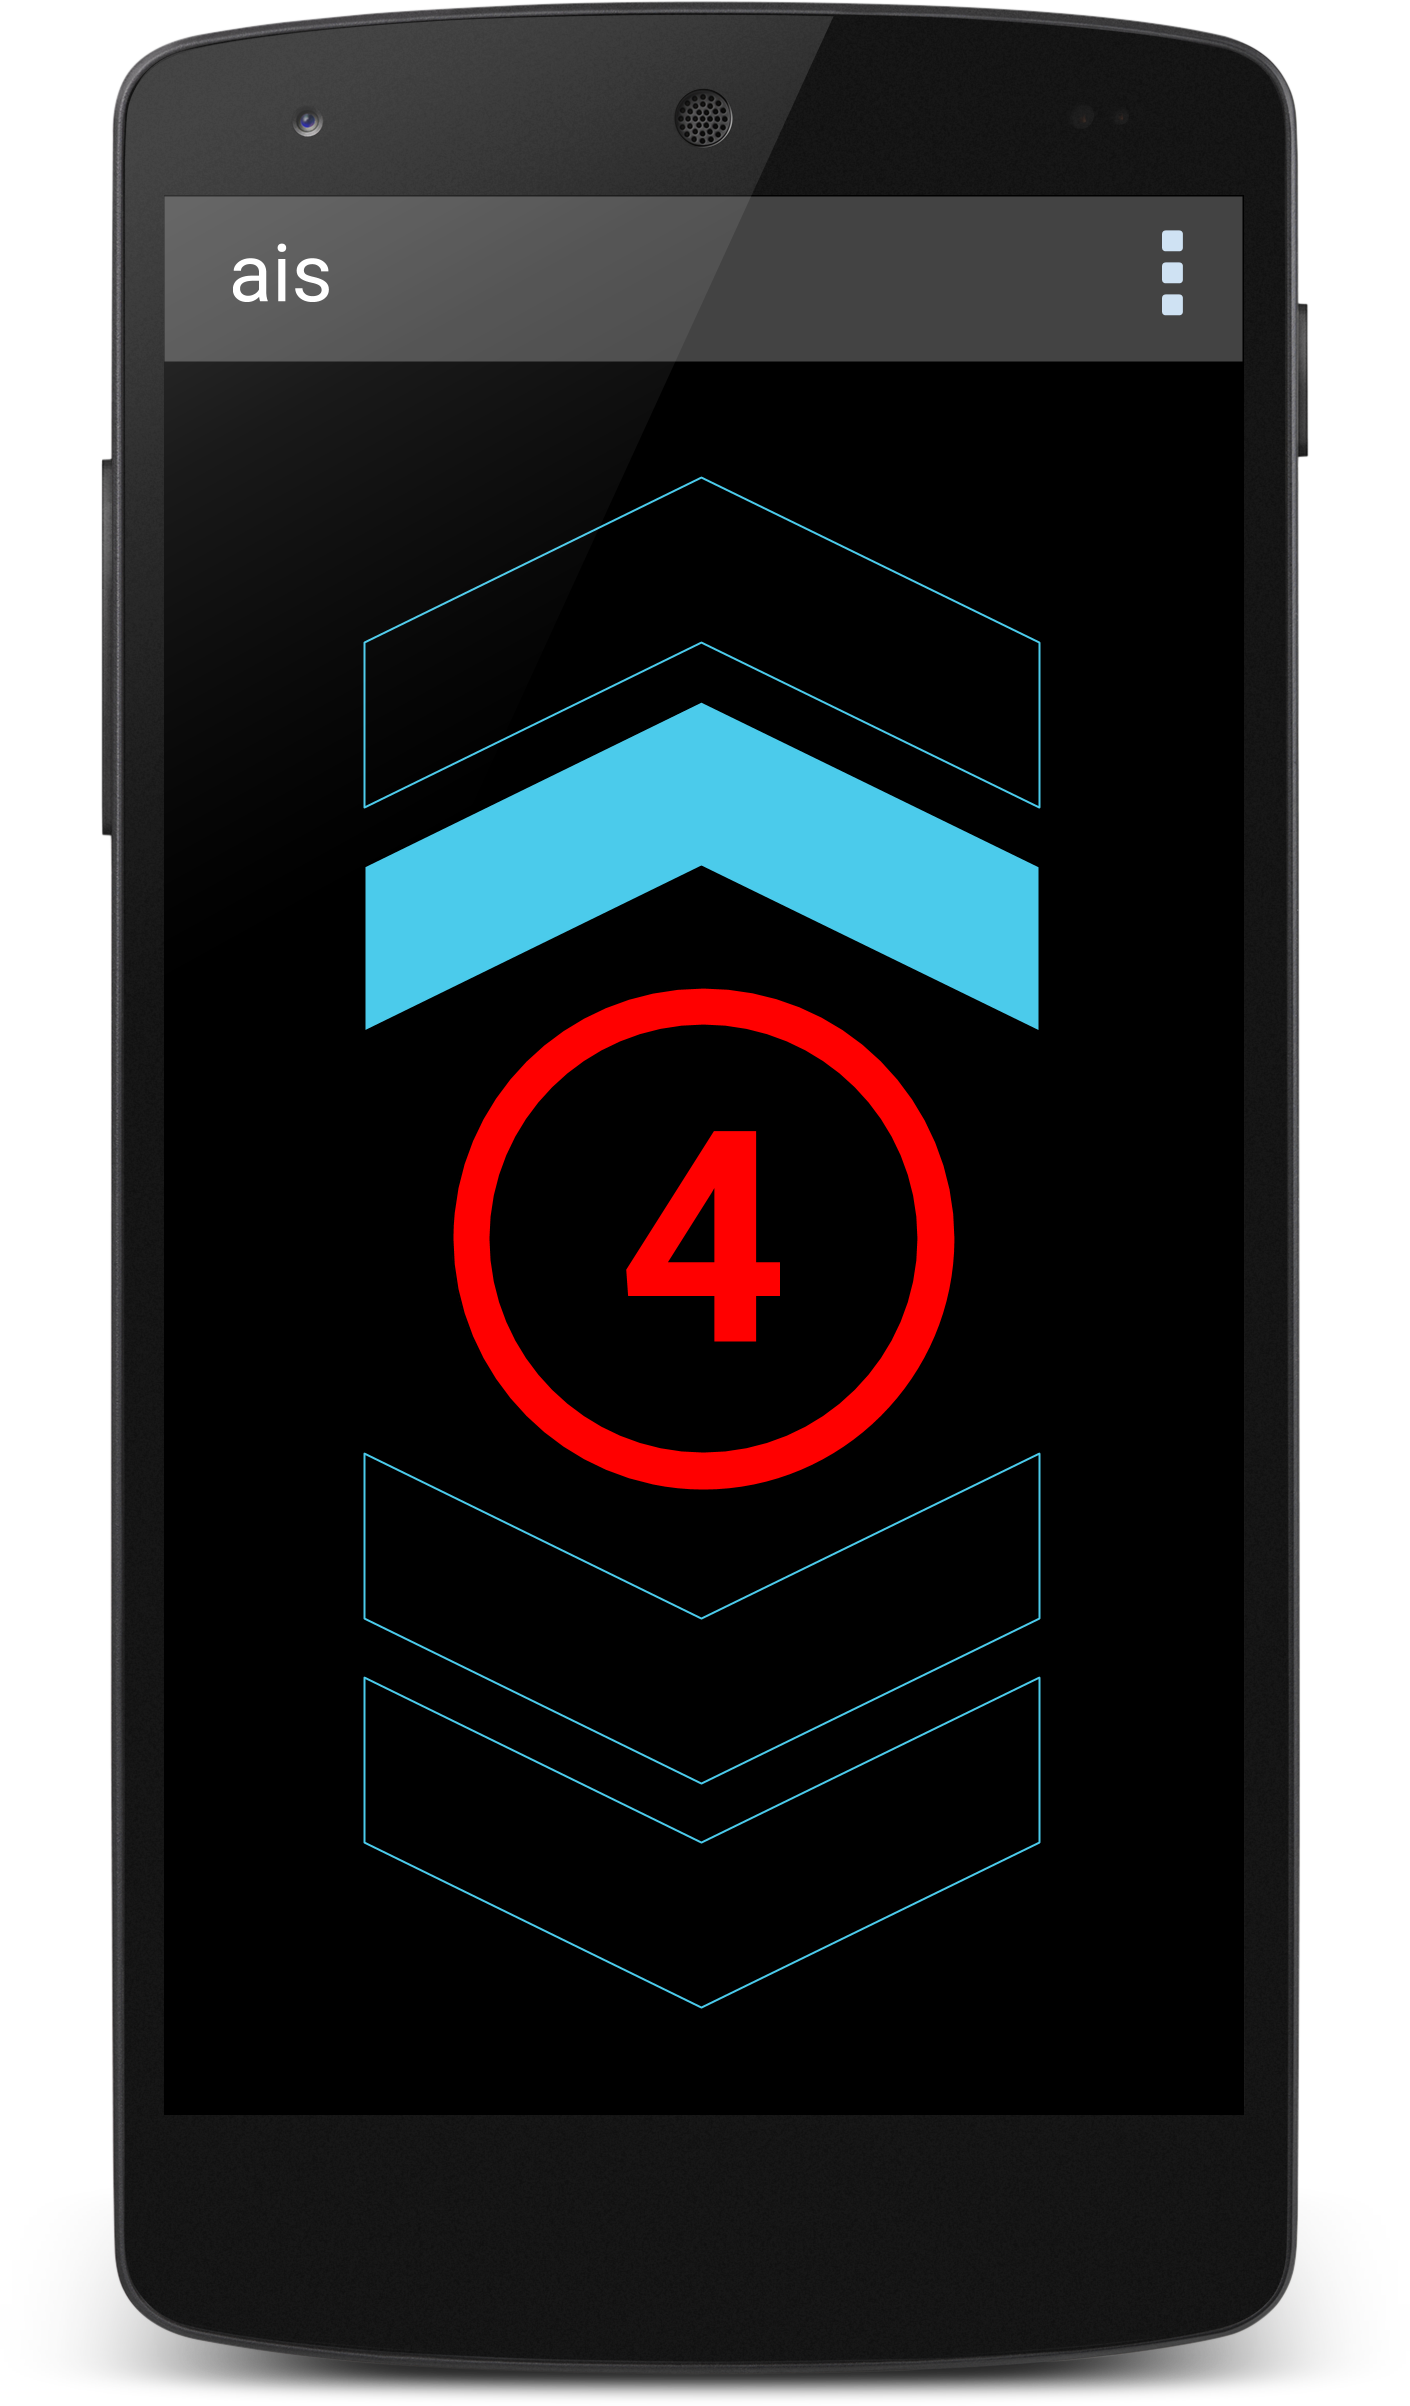
\includegraphics[width=\textwidth]{schneller}
                \caption[Systemzustand b]{Weiterfahrt durch Beschleunigung möglich}
                \label{fig:schneller}
        \end{subfigure}
        \begin{subfigure}[t]{0.36\textwidth}
                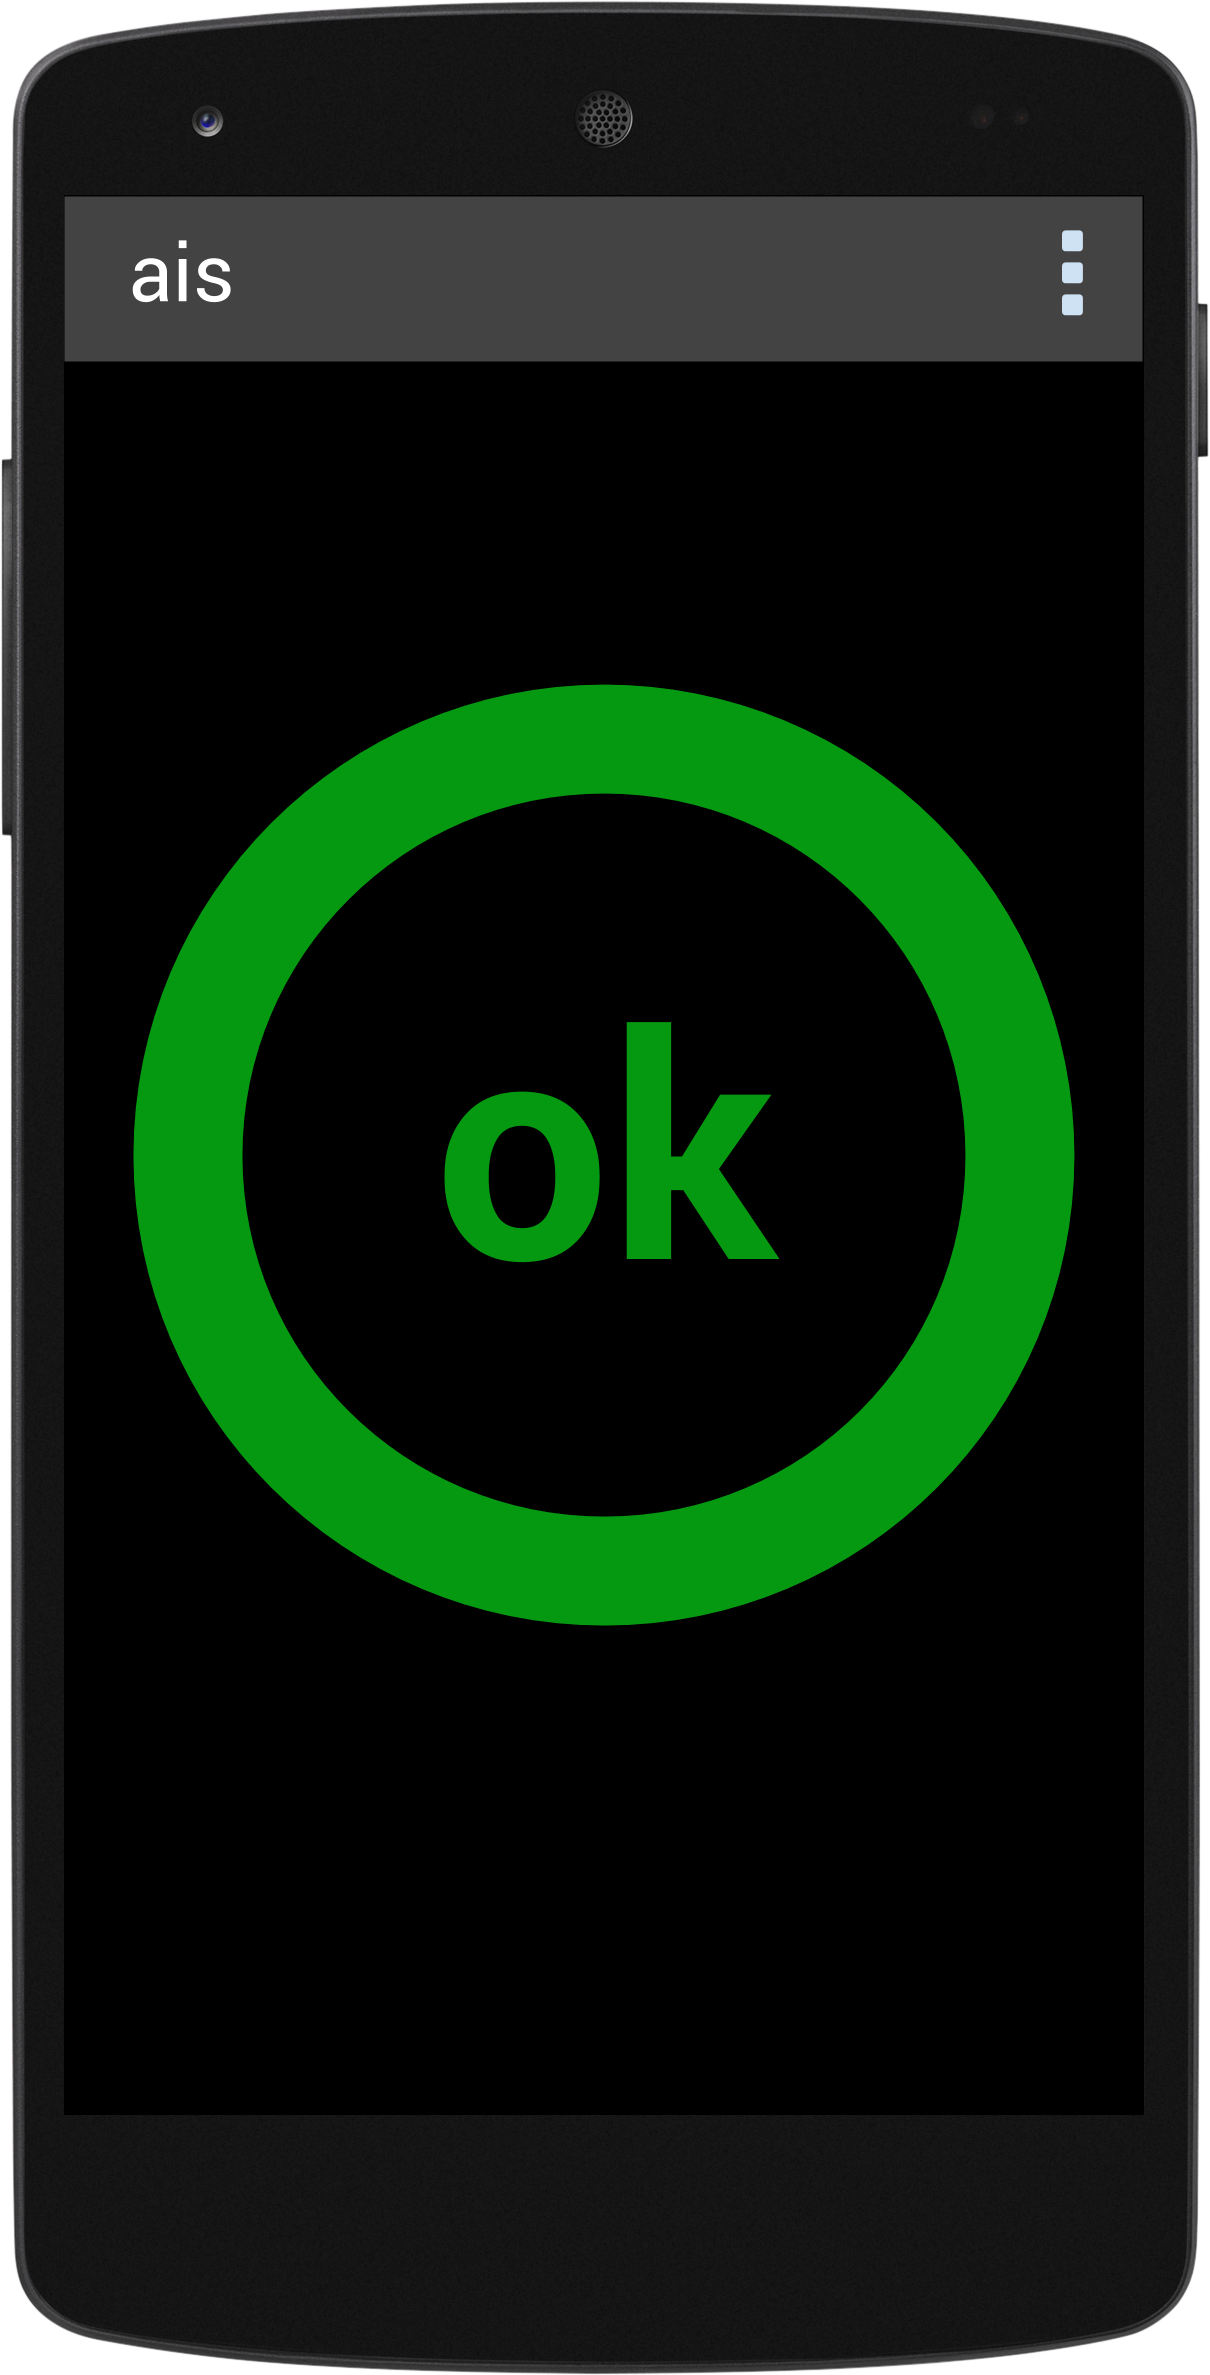
\includegraphics[width=\textwidth]{yeah1}
                \caption[Systemzustand c]{Kein Aktionsbedarf}
                \label{fig:langsamer}
        \end{subfigure}
        \hfill 
        \begin{subfigure}[t]{0.36\textwidth}
                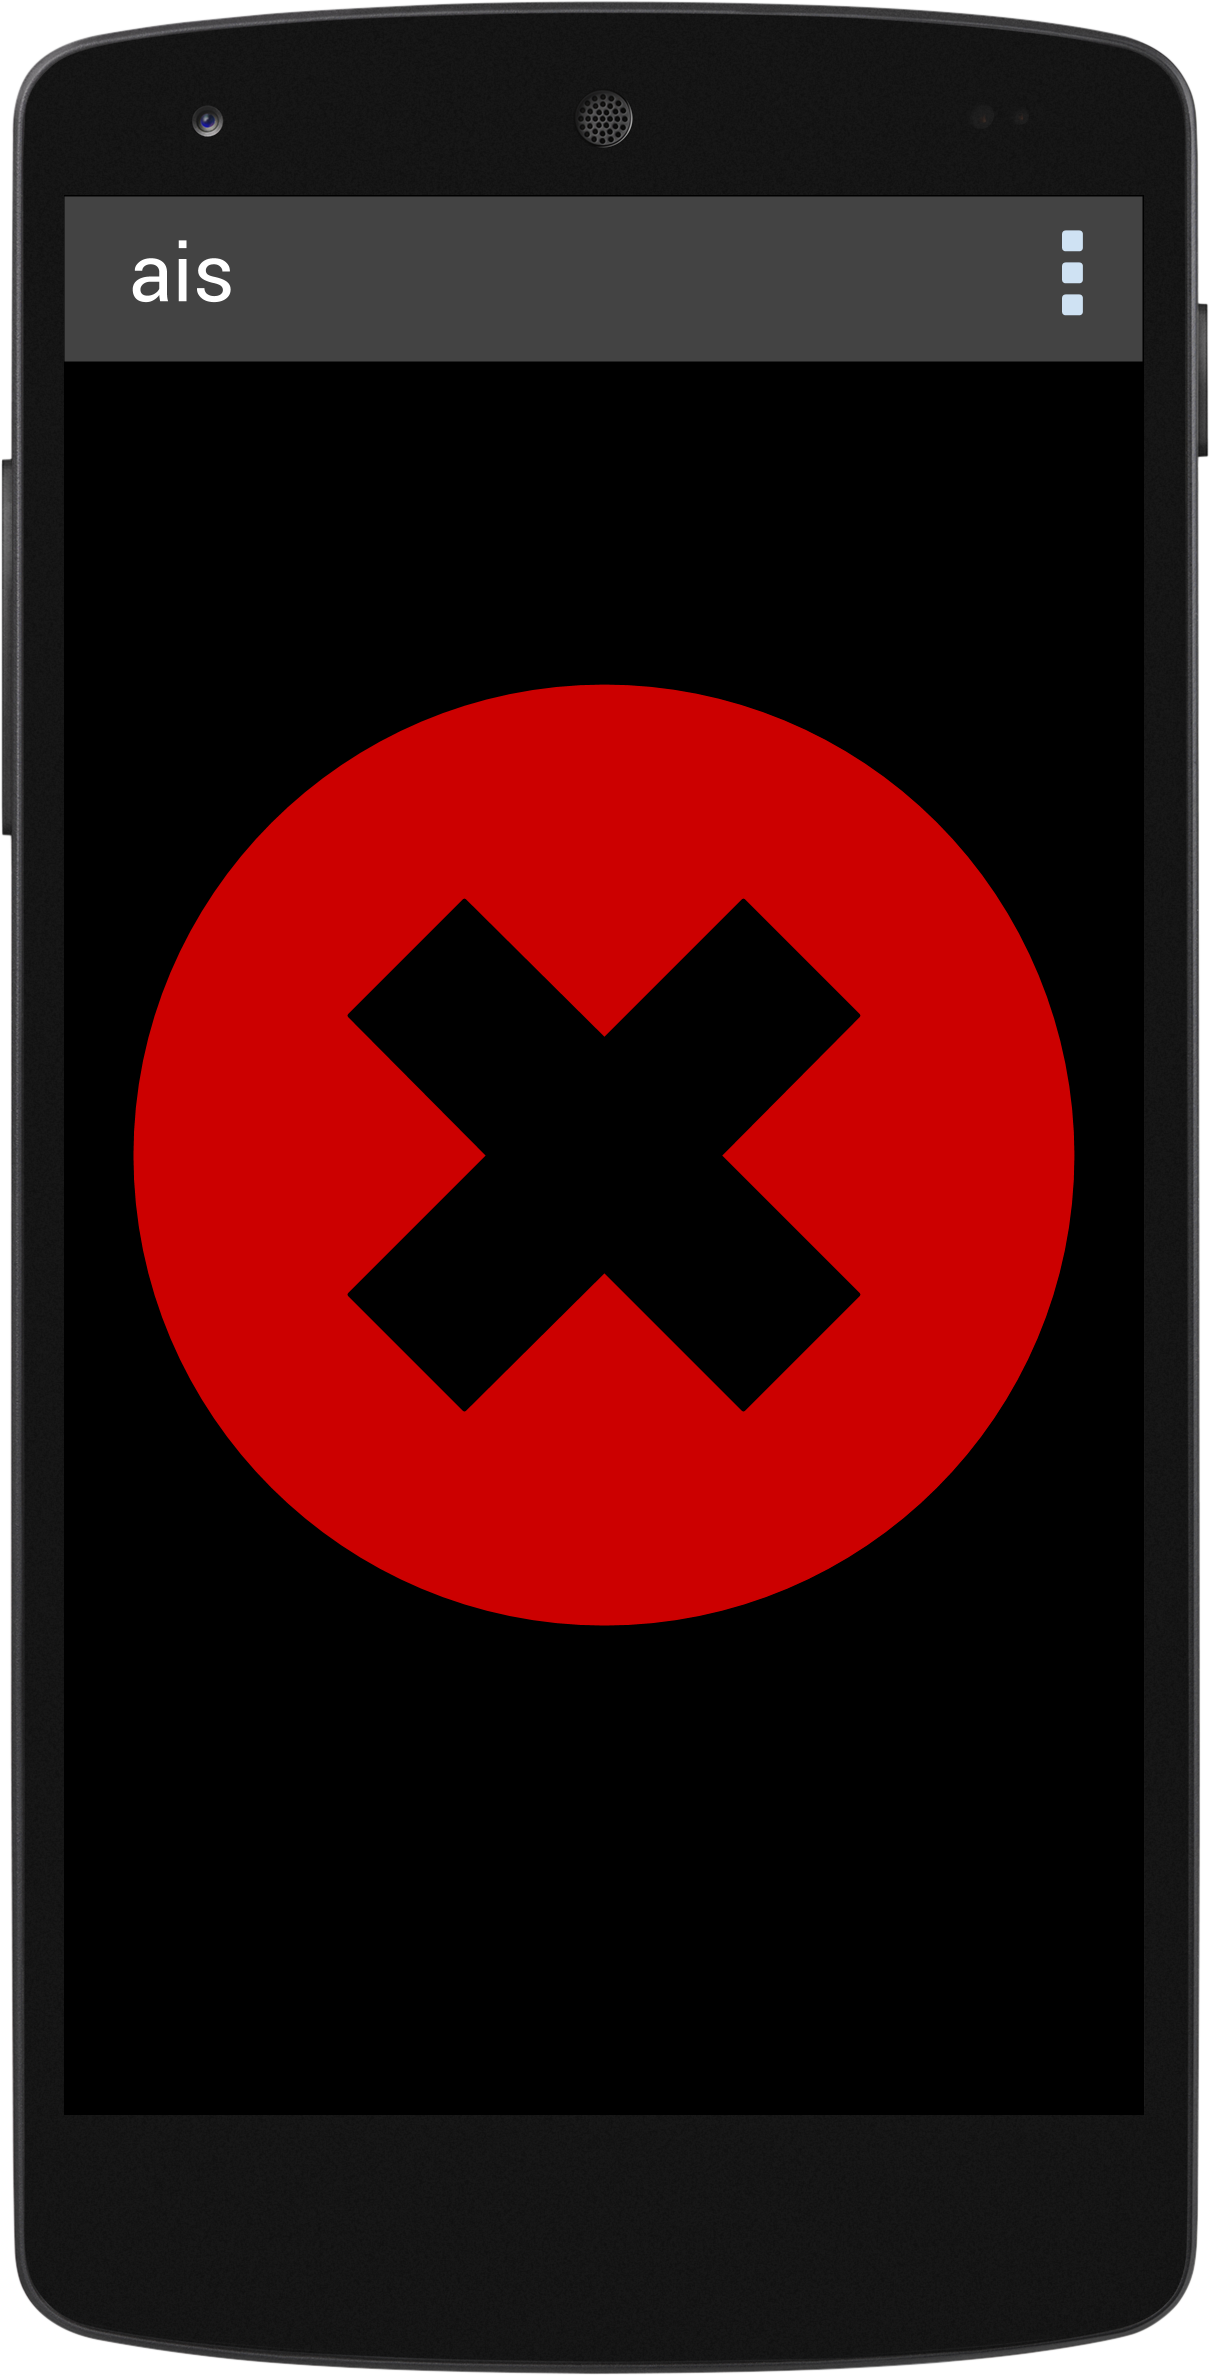
\includegraphics[width=\textwidth]{stop1}
                \caption[Systemzustand s]{keine Weiterfahrt möglich}
                \label{fig:schneller}
        \end{subfigure}
        \caption[Systemzustände im Ampelbereich]{Designkonzept Szenarien im Ampelbereich}
        \label{fig:szenario_mockup}
\end{figure} 

\section{Funktionalität} 
\section{Diagramme}
\subsection*{Sequenzdiagramm}
\subsection*{Ablaufdiagramm}
\subsection*{UML -- Diagramm}
